\documentclass[11pt]{article}
\usepackage[margin=1in]{geometry}
\usepackage{amsmath,amssymb,amsthm}
\usepackage{booktabs}
\usepackage{enumitem}
\usepackage{hyperref}
\usepackage{graphicx}
\usepackage{float}
\usepackage{array}
\usepackage{multirow}
\usepackage{xcolor}

\graphicspath{{figures/}}

\title{\textbf{Dynamic Congestion in Theme Park Queuing Networks:\\ A Stochastic Congestion Game Simulation}}
\author{Evan Cantwell, Tanay Dalmia, Zubayer Mahbub\\[4pt]\textit{ORF 387: Networks --- Spring 2026 Final Report}}
\date{}

\begin{document}
\maketitle

%----------------------------------------------------------------------
\begin{abstract}
\noindent We model Universal Studios' Epic Universe as a stochastic congestion game on a directed weighted graph and quantify how five virtual queue strategies --- free Preselect, paid Preselect, timed-slot Preselect, dynamic on-demand, and Universal-style Express --- affect aggregate visitor utility under both perfectly-rational and bounded-rational agent populations. Three findings emerge. First, targeted-allocation mechanisms (Preselect's top-3 selection) consistently outperform blanket-allocation mechanisms (Express's any-ride access) on both system happiness and the holder/non-holder fairness gap. Second, the strategy ranking is not invariant to rationality assumptions: Express climbs from third-best under perfect rationality to second-best under realistic bounded rationality, while Dynamic collapses from second to a near-tie with the no-passes baseline because its threshold rule depends on accurate wait-time perception that bounded-rational agents lack. Third, the welfare-maximizing Express adoption rate under realistic rationality assumptions is approximately 40\%, closely matching real-world Universal Express pricing that targets a similar adoption level. The work suggests that the \emph{robustness profile} of a virtual queue mechanism under bounded rationality is as important to deployment decisions as its efficiency under perfect rationality.
\end{abstract}

%----------------------------------------------------------------------
\section{Motivation, Vision, and Problem Statement}
%----------------------------------------------------------------------

Theme parks are among the most complex real-world instances of a networked congestion game. Thousands of utility-maximizing agents --- park visitors --- traverse a spatial network of attractions connected by pathways, each simultaneously choosing destinations based on incomplete information about the system state. The result is a decentralized, emergent equilibrium that is, in general, far from socially optimal --- producing systemic waste in the form of avoidable waiting.

\textbf{Central research question.} How do congestion, stochastic arrivals, and different queuing strategies jointly influence equilibrium behavior and systemic efficiency in networked theme park queuing environments? Specifically, can virtual queue interventions --- skip-the-line passes, timed reservations, and on-demand queue-skipping --- increase aggregate visitor happiness compared to a standard first-come-first-served (FCFS) baseline, and how do those gains depend on whether visitors are perfectly rational?

\textbf{Practical stakes.} Virtual queue systems at Disney World (Lightning Lane) and Universal Studios (Express Pass) have repeatedly underperformed expectations or caused visitor backlash. Disney famously discontinued the free FastPass+ system in 2021 after years of evidence that universal access caused booking-window arbitrage to dominate the experience. Quantifying \emph{why} some strategies work better than others --- and which are robust to imperfect agents --- is directly relevant to operations decisions in real parks.

\textbf{Case study.} We apply this framework to Universal Studios' \textbf{Epic Universe} (opened May 2025), a new park with five themed lands, eleven major ride attractions, and a hub-and-spoke spatial layout. Its recency provides a genuine modeling challenge while its scale produces rich congestion dynamics.

\textbf{Course topics applied.}
\begin{itemize}[nosep]
    \item \textbf{Congestion games and potential functions} (Easley \& Kleinberg, Ch.~8): The park is formally a weighted congestion game where edge costs (wait times) are non-decreasing functions of flow. Rosenthal's theorem guarantees convergence to a pure-strategy Nash equilibrium under best-response dynamics, which we implement via sequential best-response within each timestep.
    \item \textbf{Price of Anarchy} (Ch.~8): We measure the gap between the decentralized equilibrium and the system-optimal allocation that a centralized planner could in principle achieve, providing a quantitative frame for the cost of selfish routing in this setting.
    \item \textbf{Shortest-path routing} (Ch.~3): Agents use Dijkstra's algorithm on the directed park graph to compute travel times when making ride selection decisions.
    \item \textbf{Informational cascades} (Ch.~16): One of our agent behavior modes (\texttt{info\_restricted}) instantiates the chapter's central mechanism: agents make decisions from delayed wait-time signals, which compounds congestion and degrades several otherwise-efficient queue strategies.
\end{itemize}

%----------------------------------------------------------------------
\section{Model and Mathematical Framework}
%----------------------------------------------------------------------

\subsection{Network Model}

We represent Epic Universe as a weighted directed graph $G = (V, E)$ where the node set $V = V_H \cup V_A$ consists of \textbf{hub nodes} $V_H$ (themed land centers) and \textbf{attraction nodes} $V_A$ (individual rides).

\begin{itemize}[nosep]
    \item $|V_H| = 5$ hub nodes: Celestial Park (central hub), Super Nintendo World, Dark Universe, Wizarding World, Isle of Berk.
    \item $|V_A| = 11$ attraction nodes: the queue-based rides with published capacity and wait-time data.
    \item Total: $|V| = 16$ nodes, $|E| = 30$ directed edges.
\end{itemize}

\textbf{Hub-and-spoke topology.} All inter-land travel must route through Celestial Park, matching the real park's portal system. There are no direct connections between themed lands.

\textbf{Edge cost structure.}

\begin{table}[H]
\centering
\begin{tabular}{llll}
\toprule
\textbf{Edge Type} & \textbf{Direction} & \textbf{Weight} & \textbf{Count} \\
\midrule
Hub-to-hub (walkways) & Bidirectional & $c_e = d_e$ (walking time, min) & 8 \\
Hub-to-attraction (ride entrance) & Hub $\to$ Ride & $c_e = 1$ min & 11 \\
Attraction-to-hub (ride exit) & Ride $\to$ Hub & $c_e = 1$ min & 11 \\
\bottomrule
\end{tabular}
\end{table}

Hub-to-hub distances were measured as straight-line distances between land centers using Google Earth satellite imagery and converted to walking time at 80 m/min ($\approx$~3 mph).

\subsection{Attraction Data and Enjoyment Scores}

All ride data was manually verified from thrill-data.com lifetime summary statistics. For each of the 11 rides, we collected average wait time, theoretical hourly capacity, and ride duration from multiple theme park databases.

\textbf{Enjoyment score derivation.} Raw wait time alone does not capture true popularity because high-capacity rides process more visitors with shorter waits. We estimate underlying demand using Little's Law:
\[
\bar{Q}_a = \bar{W}_a \cdot \frac{\mu_a}{60}
\]
where $\bar{W}_a$ is the lifetime average wait (minutes) and $\mu_a$ is hourly capacity (riders/hour). The enjoyment score is then log-normalized to a 1--10 scale:
\[
h_a = 1 + 9 \cdot \frac{\ln \bar{Q}_a - \ln \bar{Q}_{\min}}{\ln \bar{Q}_{\max} - \ln \bar{Q}_{\min}}.
\]

\textbf{Capacity conversion.} Per-cycle capacity is derived from hourly throughput:
\[
C_a = \text{round}\!\left(\mu_a \cdot \frac{s_a}{60}\right)
\]
where $s_a$ is the ride duration in minutes.

\subsection{Agent Model and Utility Function}

We model $N \approx 20{,}000$ agents (park visitors) per simulated day. Each agent $i$ has a heterogeneous personal preference vector drawn at creation:
\[
\text{pref}_{ia} \sim \max\!\big(0.1,\; \mathcal{N}(1.0,\, 0.3)\big) \quad \forall\, a \in V_A.
\]

\textbf{Utility function.} At each decision point, agent $i$ evaluates every ride $a$ using:
\[
U_i(a, t) = \frac{h_a \cdot \text{pref}_{ia} \cdot \gamma_i(t) \cdot r_{ia}}{\sqrt{1 + W_i(a, t) + D(v_i, a)}}
\]
where:
\begin{itemize}[nosep]
    \item $h_a$ is the ride's enjoyment score (1--10), derived from real data.
    \item $\text{pref}_{ia}$ is the agent's personal preference multiplier.
    \item $\gamma_i(t) = (T_{\text{dep},i} - t) / (T_{\text{dep},i} - T_{\text{arr},i})$ is a linear time-decay factor.
    \item $r_{ia} = 1 / (1 + 0.5\, n_{ia})$ is a diminishing-returns factor for re-rides on attraction $a$.
    \item $W_i(a, t)$ is the wait time agent $i$ would actually face for ride $a$ at time $t$ (see \S2.4).
    \item $D(v_i, a)$ is the shortest-path travel time from agent $i$'s current node to $a$, computed via Dijkstra.
\end{itemize}

The $\sqrt{1 + W + D}$ denominator ensures that utility is always non-negative and that wait/travel impose diminishing rather than absolute penalties. An earlier subtractive formulation $U = H - W - D$ caused agents to leave the park after 4--5 rides because the 1--10 enjoyment scale could not compete with wait times of 30--100 minutes.

Agent $i$ selects $a^* = \arg\max_{a \in V_A} U_i(a, t)$, subject to the feasibility constraint $D + W + s_a \leq T_{\text{dep},i} - t$. If no ride yields positive utility, the agent departs the park early.

\subsection{Wait Time Model}

Each ride node maintains two queues: a regular FIFO queue and a separate priority queue for pass holders. Each ride cycle drains the priority queue first up to capacity, with any remaining capacity drawn from the regular queue. Because these two queues face different effective wait times, we resolve $W_i(a, t)$ against the queue agent $i$ would actually enter:
\begin{align*}
W_{\text{priority}}(a, t) &= \frac{|\text{priority\_queue}(a, t)|}{C_a} \cdot s_a \\[4pt]
W_{\text{regular}}(a, t) &= \frac{|\text{priority\_queue}(a, t)| + |\text{regular\_queue}(a, t)| + p_a(t)}{C_a} \cdot s_a
\end{align*}
where $p_a(t)$ is the number of agents who have committed to ride $a$ but are still in transit (the \emph{pending arrivals} counter). The regular-queue wait correctly reflects that regular-queue agents are blocked behind the entire priority queue ahead of them, since priority drains first each cycle.

When agent $i$ has an available pass for ride $a$, $W_i(a, t) = W_{\text{priority}}(a, t)$. Otherwise $W_i(a, t) = W_{\text{regular}}(a, t)$. For agents with the \texttt{info\_restricted} behavior (\S2.5), $W$ is read instead from a 15-minute-stale shared wait-time board that reflects $W_{\text{regular}}$; pass-holder priority wait is approximated as zero in that case because the stale board does not expose priority queue lengths.

\subsection{Agent Behaviors}

Each agent carries a (possibly empty) subset of behavior flags that modify decision-making. Behaviors compose: any subset can be active simultaneously per simulation. The empty set defines a \emph{perfectly rational} agent.

\begin{itemize}[nosep]
    \item \textbf{\texttt{fatigue}}: switching away from the previously-committed ride target requires a $\geq 5\%$ utility improvement. Models the cognitive cost of changing one's mind mid-decision.
    \item \textbf{\texttt{info\_restricted}}: agent uses a 15-minute-stale wait-time board instead of live queue lengths. This is the chapter-16 informational cascades mechanism: delayed signals cause herding behavior that compounds congestion.
    \item \textbf{\texttt{proximity\_bias}}: utility multiplied by $0.95^{D / 0.5}$, so every additional 30 seconds of travel costs 5\%. Models agents over-weighting walking distance.
    \item \textbf{\texttt{decision\_paralysis}}: agents draw $\text{decision\_speed} \in \{0, 1, 2, 4\}$ minutes uniformly at creation. When a decision is a near-tie (two or more rides within 5\% of the chosen utility), the agent stalls for $\text{decision\_speed}$ minutes before committing.
    \item \textbf{\texttt{eating\_resting}}: hunger-driven meal breaks. Each agent draws a hunger threshold from $\text{clip}(\mathcal{N}(225, 15), 180, 270)$ minutes. When time-since-last-meal crosses the threshold (and at least 32 minutes remain before departure), the agent walks to its land's hub and rests for $\text{clip}(\mathcal{N}(30, 5), 25, 35)$ minutes before resuming ride selection.
\end{itemize}

\subsection{Pass Strategies}

We compare five virtual queue strategies plus the FCFS baseline:

\begin{itemize}[nosep]
    \item \textbf{\texttt{none}} (FCFS baseline): no skip-the-line mechanism.
    \item \textbf{\texttt{preselect}} (free, anytime): every agent receives 3 anytime passes for their personal top-3 rides (ranked by $h_a \cdot \text{pref}_{ia}$). Models the legacy Disney FastPass+ system.
    \item \textbf{\texttt{preselect\_paid}}: same mechanic, but only an adopter fraction $\alpha$ receives the 3 passes. The remaining $(1 - \alpha)$ guests have no skip access. Models a hypothetical paid Disney-style anytime pass.
    \item \textbf{\texttt{preselect\_timed}}: same top-3 selection but each pass is bound to an assigned 5-minute time window (round-robin across 144 windows per ride per day, with a 30-minute minimum gap between an agent's three passes). Models Disney's previous FastPass+ time-locked mechanism.
    \item \textbf{\texttt{dynamic}}: each agent receives 3 unassigned passes used adaptively when the perceived wait at a chosen ride exceeds 30 minutes.
    \item \textbf{\texttt{express}}: an adopter fraction $\beta$ receives an Express Pass that grants priority access to every ride in the park, used once per ride. Models Universal Orlando's Express Pass. For simplicity, our implementation allows Express on every attraction; the real Universal product excludes Dragon Racer's Rally.
\end{itemize}

All pass mechanisms route holders into the priority queue at the target ride. Priority queues drain first each cycle up to capacity; any remaining capacity is drawn from the regular queue.

\subsection{Arrival and Departure Dynamics}

\textbf{Arrival model.}
\begin{enumerate}[nosep]
    \item \textbf{Gate rush}: 3,000 agents arrive during the first 30 minutes with inter-arrival times drawn from $\text{Exp}(\lambda = 1/5)$ minutes, clipped to $[0, 30]$.
    \item \textbf{Steady state}: From $t = 30$ to $t = 720$ (park close), new agents arrive each minute at rate $\text{Poisson}(17{,}000 / 690 \approx 24.6)$. Total steady-state arrivals $\approx 17{,}000$.
\end{enumerate}
Combined daily attendance: $\approx 20{,}000$ agents, consistent with reported Epic Universe averages of 16,000--22,000.

\textbf{Departure model.} Each agent's planned departure time $T_{\text{dep},i} \sim \mathcal{N}(600, 60)$ minutes from park open, clipped to $[T_{\text{arr},i} + 60,\, 720]$. Agents also depart early if no ride has positive utility.

\subsection{Simulation Architecture}

The simulation is a discrete-time agent-based model with timestep $\Delta t = 1$ minute, running for 720 steps (9:00 AM to 9:00 PM). Each timestep executes seven sequential phases: arrivals, ride processing, departures, decisions (sequential best-response), travel, rest tick, and wait/hunger accounting. The Phase~4 decision step shuffles deciding agents and processes them one at a time; each commitment increments the target ride's \emph{pending arrivals} counter, so subsequent agents within the same timestep see an updated wait estimate. Under this process, the Rosenthal potential function $\Phi(x) = \sum_{e} \sum_{k=1}^{x_e} c_e(k)$ is monotonically non-increasing under improvement moves, guaranteeing convergence to a pure-strategy Nash equilibrium (Easley \& Kleinberg, Theorem~8.3).

%----------------------------------------------------------------------
\section{Data Sources and Calibration}
%----------------------------------------------------------------------

\subsection{Data Sources}

\begin{table}[H]
\centering
\begin{tabular}{p{3.5cm}p{5cm}p{5cm}}
\toprule
\textbf{Source} & \textbf{Data Collected} & \textbf{Use in Model} \\
\midrule
thrill-data.com (lifetime stats) & Average wait times, hourly capacity for all 11 rides & Enjoyment scores $h_a$, service rates $\mu_a$ \\
Google Earth satellite imagery & Straight-line distances between 5 land centers & Hub-to-hub edge weights \\
orlandoinformer.com, undercovertourist.com, frommers.com, attractionsmagazine.com & Ride durations (1.5--5 min per ride) & Cycle time $s_a$ \\
thrill-data.com, disneytouristblog.com & Daily attendance estimates (16,000--22,000) & Total agent count $N$ \\
\bottomrule
\end{tabular}
\end{table}

\subsection{Attraction Parameter Table}

\begin{table}[H]
\centering
\small
\begin{tabular}{lcccccc}
\toprule
\textbf{Attraction} & \textbf{Land} & $\bar{W}_a$ & $\mu_a$ & $s_a$ & $C_a$ & $h_a$ \\
 & & (min) & (riders/hr) & (min) & (per cycle) & \\
\midrule
Harry Potter Battle at Ministry$^*$ & Wizarding & 90 & 2,184 & 4.5 & 164 & 10.0 \\
Hiccup's Wing Gliders & Isle of Berk & 62 & 1,800 & 2.0 & 60 & 8.4 \\
Mario Kart: Bowser's Challenge & Super Nintendo & 96 & 1,100 & 4.0 & 73 & 8.2 \\
Stardust Racers & Celestial Park & 38 & 2,700 & 1.5 & 68 & 8.1 \\
Mine-Cart Madness & Super Nintendo & 116 & 750 & 2.0 & 25 & 7.7 \\
Monsters Unchained & Dark Universe & 29 & 2,400 & 4.0 & 160 & 7.0 \\
Curse of the Werewolf & Dark Universe & 54 & 750 & 2.0 & 25 & 5.4 \\
Yoshi's Adventure & Super Nintendo & 45 & 675 & 5.0 & 56 & 4.6 \\
Fyre Drill & Isle of Berk & 30 & 600 & 3.5 & 35 & 3.1 \\
Dragon Racer's Rally & Isle of Berk & 45 & 275 & 1.5 & 7 & 2.0 \\
Constellation Carousel & Celestial Park & 18 & 480 & 2.0 & 16 & 1.0 \\
\bottomrule
\end{tabular}
\caption{Attraction parameters for the 11 modeled rides. $^*$Harry Potter's observed lifetime average wait is 135 min under actual operations ($\sim$1,450 riders/hr). We adjusted to 90 min to match optimal theoretical capacity (2,184 riders/hr), since our simulation assumes all rides run at full capacity throughout the day.}
\end{table}

\subsection{Modeling Assumptions}

The simulation rests on a number of explicit assumptions that shape the interpretation of our results.

\textbf{Operations.}
\begin{itemize}[nosep]
    \item All rides run continuously at theoretical hourly capacity with no downtime, mechanical issues, or staffing constraints. This represents a best-case operational scenario.
    \item Park operating hours are 9:00 AM to 9:00 PM; we do not model variation in operating hours across days of the week or seasons.
\end{itemize}

\textbf{Spatial.}
\begin{itemize}[nosep]
    \item All rides within a themed land are co-located at the land's hub; the walking time from a hub to any of its rides is 1 minute. Real intra-land variation (some rides are deeper into the land than others) is not captured.
    \item Inter-land travel must route through Celestial Park; no shortcuts. This matches the real portal layout.
    \item Hub-to-hub distances are straight-line measurements from Google Earth, converted at 3 mph. Real walking paths are 20--40\% longer due to curvature.
\end{itemize}

\textbf{Agent and decision.}
\begin{itemize}[nosep]
    \item Agents are individuals making independent decisions. Real visitors travel in family or friend groups whose preferences must be reconciled.
    \item The multiplicative utility form, with the $\sqrt{1 + W + D}$ denominator, was selected over a subtractive form because the latter caused unrealistic early departures; the tradeoff is reduced sensitivity to large differences in wait time.
    \item The hyperbolic re-ride decay $1/(1 + 0.5n)$ was chosen over a steeper exponential because the exponential exhausted re-ride utility too quickly.
    \item Agents' personal preferences follow $\mathcal{N}(1.0, 0.3)$, floored at 0.1, giving 30\% relative variation while preserving roughly-shared rankings.
\end{itemize}

\textbf{Ride-specific calibration.}
\begin{itemize}[nosep]
    \item Battle at the Ministry's wait time was scaled from 135 min (observed) to 90 min (theoretical-capacity equivalent) to avoid inflating its demand relative to other rides not subject to similar operational issues.
    \item Mine-Cart Madness's ride duration is a 2-minute estimate; no published value was located.
    \item Fyre Drill's hourly capacity (600/hr) is user-provided; published sources do not list it.
    \item 14 non-ride attractions (meet-and-greets, shows, open play areas) are excluded from the simulation graph because reliable wait-time and capacity data are unavailable.
\end{itemize}

\textbf{Out-of-scope.} The model does not capture weather, ride breakdowns, multi-day visitors, dynamic pricing, or group-decision dynamics.

%----------------------------------------------------------------------
\section{Results}
%----------------------------------------------------------------------

We organize results in six subsections: baseline calibration, strategy comparison under perfect rationality, strategy comparison under bounded rationality, an Express Pass adoption sweep, a paid Preselect adoption sweep, and a dedicated fairness analysis.

\subsection{Baseline Calibration}

The no-passes baseline (\texttt{none}, no behaviors active) produces emergent behavior consistent with reported Epic Universe operations:

\begin{table}[H]
\centering
\begin{tabular}{lc}
\toprule
\textbf{Metric} & \textbf{Value} \\
\midrule
Total agents generated & $\sim$20,000 \\
Peak in-park population & $\sim$13,800 (5:00 PM) \\
Avg rides completed per agent & 8.10 \\
Avg total wait time per agent & 256.1 min \\
Most congested ride & Harry Potter \\
\bottomrule
\end{tabular}
\caption{Baseline simulation metrics, mean of 3 random seeds (\texttt{none} pass strategy, no behaviors active).}
\end{table}

The simulated congestion ranking matches real-world observations: Harry Potter, Hiccup's Wing Gliders, and Mario Kart are the three most congested attractions. Per-ride waits average $\sim$32 minutes (256 min total wait / 8 rides), which is lower than the real-world park average of $\sim$53 minutes. This is expected: rational agents with full information spread load more efficiently than real visitors who exhibit herding and information friction. Figures \ref{fig:none-queues} and \ref{fig:none-pop} show the baseline park-wide queue load and population dynamics across the day.

\begin{figure}[H]
\centering
\begin{minipage}{0.49\textwidth}
\centering
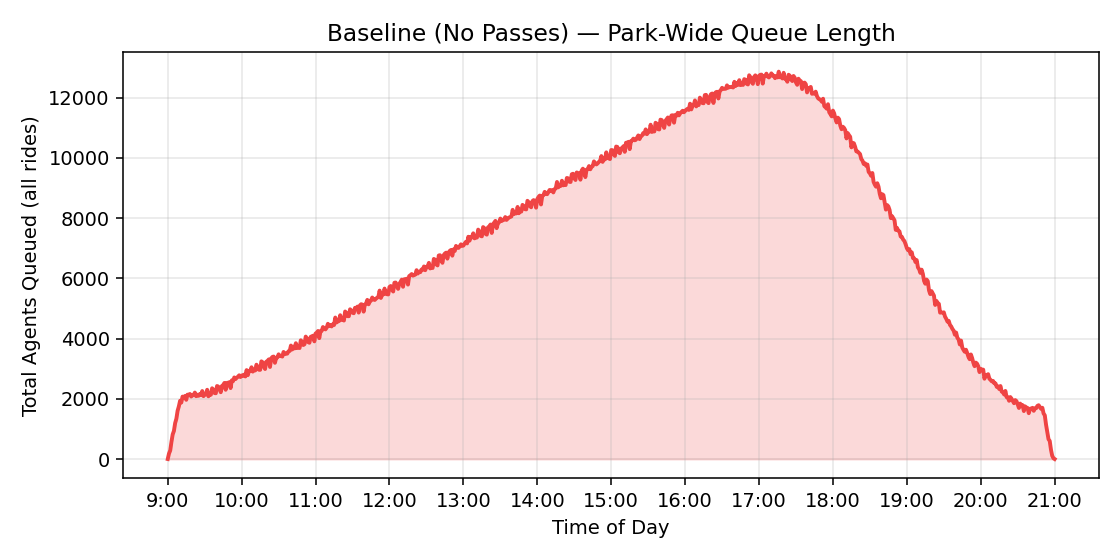
\includegraphics[width=\linewidth]{none_queues.png}
\caption{Park-wide regular-queue length over the day, baseline.}
\label{fig:none-queues}
\end{minipage}\hfill
\begin{minipage}{0.49\textwidth}
\centering
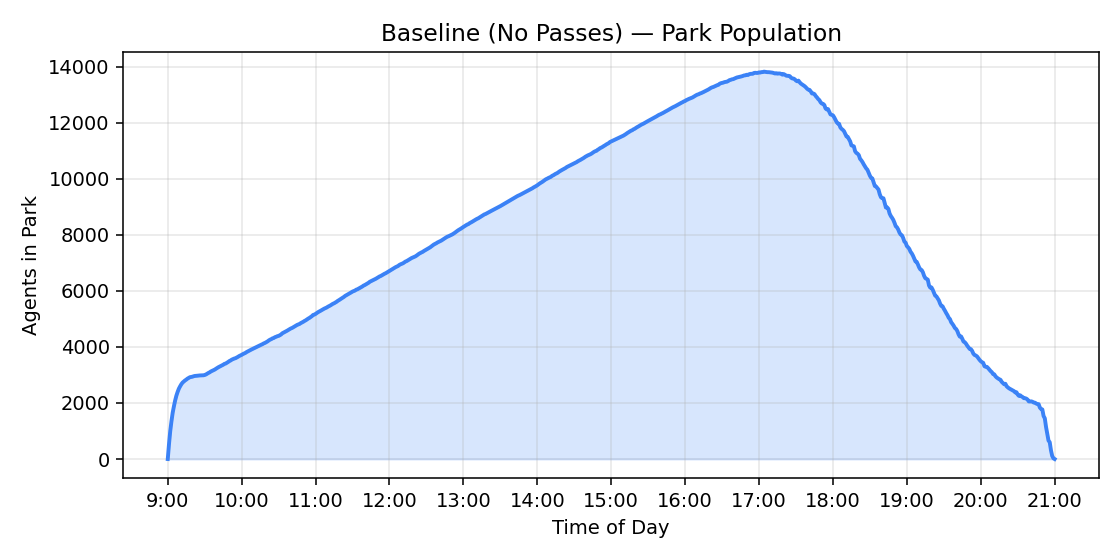
\includegraphics[width=\linewidth]{none_population.png}
\caption{In-park population over the day, baseline. Peaks at $\sim$13,800 at 5:00 PM.}
\label{fig:none-pop}
\end{minipage}
\end{figure}

\subsection{Strategy Comparison Under Perfect Rationality}

We compare the five strategies against the baseline using a 3-seed Monte Carlo simulation per strategy (seeds 42, 1, and 7) with all behaviors disabled. Table~\ref{tab:rational-strategies} reports mean and standard deviation of the per-agent average happiness, total wait, and rides completed.

\begin{table}[H]
\centering
\small
\begin{tabular}{lcccc}
\toprule
\textbf{Strategy} & \textbf{Avg Happiness} & \textbf{$\Delta$ vs Baseline} & \textbf{Avg Wait (min)} & \textbf{Avg Rides} \\
\midrule
Baseline (No Passes) & $38.03 \pm 0.21$ & --- & 256.1 & 8.10 \\
Preselect (Anytime, free) & $47.09 \pm 0.22$ & \textbf{+23.8\%} & 258.7 & 7.99 \\
Preselect (Timed Slots) & $38.54 \pm 0.20$ & +1.3\% & 262.8 & 8.14 \\
Dynamic (On-Demand) & $46.22 \pm 0.27$ & +21.5\% & 267.2 & 8.07 \\
Express Pass (30\% adoption) & $41.64 \pm 0.24$ & +9.5\% & 262.2 & 8.13 \\
\bottomrule
\end{tabular}
\caption{Strategy comparison, perfectly-rational agents, 3-seed mean $\pm$ std.}
\label{tab:rational-strategies}
\end{table}

\textbf{Observations.}
\begin{itemize}[nosep]
    \item \textbf{Free Preselect (Anytime) is the highest-utility configuration} (+23.8\%), narrowly beating Dynamic (+21.5\%). Pass holders benefit from skipping their three personally-highest-value rides.
    \item \textbf{Express @ 30\% delivers a moderate +9.5\% gain.} It is the only realistic 2026-style deployment in this set: Universal currently sells Express at \$80--300 per day specifically to limit adoption to a similar fraction.
    \item \textbf{Timed slots barely move the needle} (+1.3\%). Round-robin time-window assignment matches each agent's 3 passes to specific clock times, but agents are frequently elsewhere in the park when their window opens, leaving most timed passes unused.
\end{itemize}

\begin{figure}[H]
\centering
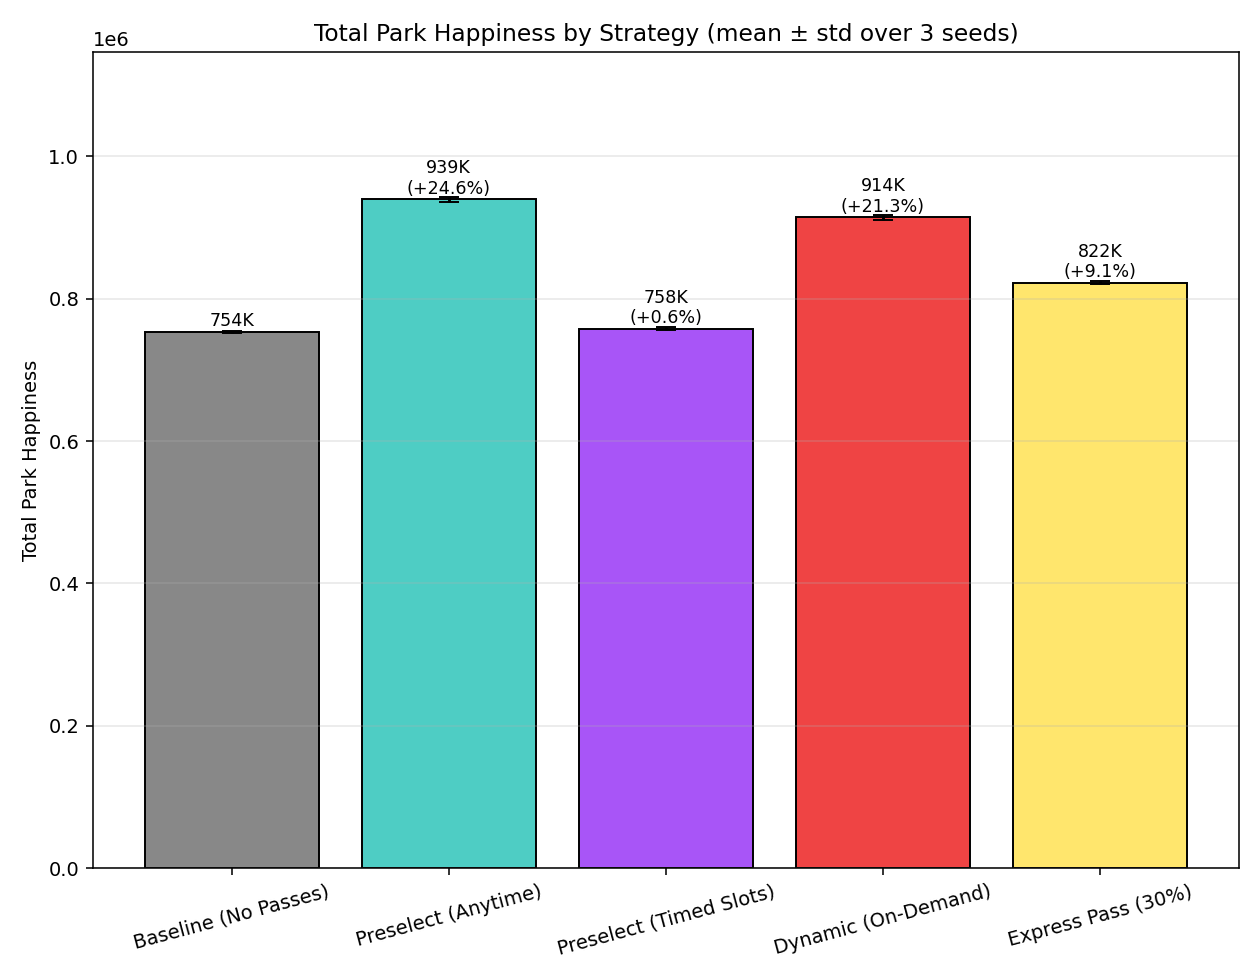
\includegraphics[width=0.9\linewidth]{comparison_happiness.png}
\caption{Total park happiness by strategy under perfect rationality (3-seed mean $\pm$ std).}
\label{fig:rational-comparison}
\end{figure}

\subsection{Strategy Comparison Under Bounded Rationality}

We repeat the strategy comparison with all five behaviors enabled simultaneously (\texttt{fatigue} + \texttt{info\_restricted} + \texttt{proximity\_bias} + \texttt{decision\_paralysis} + \texttt{eating\_resting}). Table~\ref{tab:behaviors-strategies} compares the bounded-rational outcome to the rational outcome from Table~\ref{tab:rational-strategies}.

\begin{table}[H]
\centering
\small
\begin{tabular}{lcccc}
\toprule
\textbf{Strategy} & \textbf{Behaviors avgH} & \textbf{Rational avgH} & \textbf{Robustness $\Delta$} \\
\midrule
Preselect (Anytime, free) & $45.02 \pm 0.28$ & 47.09 & $-2.07$ \\
Express Pass (30\%) & $41.23 \pm 0.13$ & 41.64 & \textbf{$-0.41$} \\
Dynamic (On-Demand) & $39.87 \pm 0.44$ & 46.22 & \textbf{$-6.35$} \\
Baseline (No Passes) & $39.27 \pm 0.20$ & 38.03 & $+1.24$ \\
Preselect (Timed Slots) & $39.20 \pm 0.21$ & 38.54 & $+0.66$ \\
\bottomrule
\end{tabular}
\caption{Strategy comparison, all behaviors enabled, 3-seed mean $\pm$ std. \textbf{Robustness $\Delta$} is the change in average happiness moving from rational to bounded-rational agents.}
\label{tab:behaviors-strategies}
\end{table}

The strategy ranking re-orders. Under perfect rationality, the order (descending happiness) was:
\[
\text{Preselect} > \text{Dynamic} > \text{Express} > \text{Timed} > \text{Baseline}.
\]
Under bounded rationality, it becomes:
\[
\text{Preselect} > \text{Express} > \text{Dynamic} \approx \text{Baseline} > \text{Timed}.
\]

\textbf{Three structural findings:}
\begin{itemize}[nosep]
    \item \textbf{Express is the most robust mechanism.} Its loss is only $-0.41$ happiness under imperfect rationality. The mechanism's "always use the pass on whatever ride you visit" rule does not require sophisticated wait-time judgment, so \texttt{info\_restricted}'s stale information has minimal effect on pass usage.
    \item \textbf{Dynamic is the most fragile.} Its loss is $-6.35$, dropping it from 2nd-best to a virtual tie with the no-passes baseline. The mechanism's 30-minute wait-threshold rule is sensitive to wait-time perception; \texttt{info\_restricted} agents cannot accurately judge when to spend a pass.
    \item \textbf{Baseline rises slightly} ($+1.24$), driven by a congestion-relief externality from \texttt{eating\_resting}: meal breaks naturally smooth peak demand, freeing capacity for non-resting agents.
\end{itemize}

\begin{figure}[H]
\centering
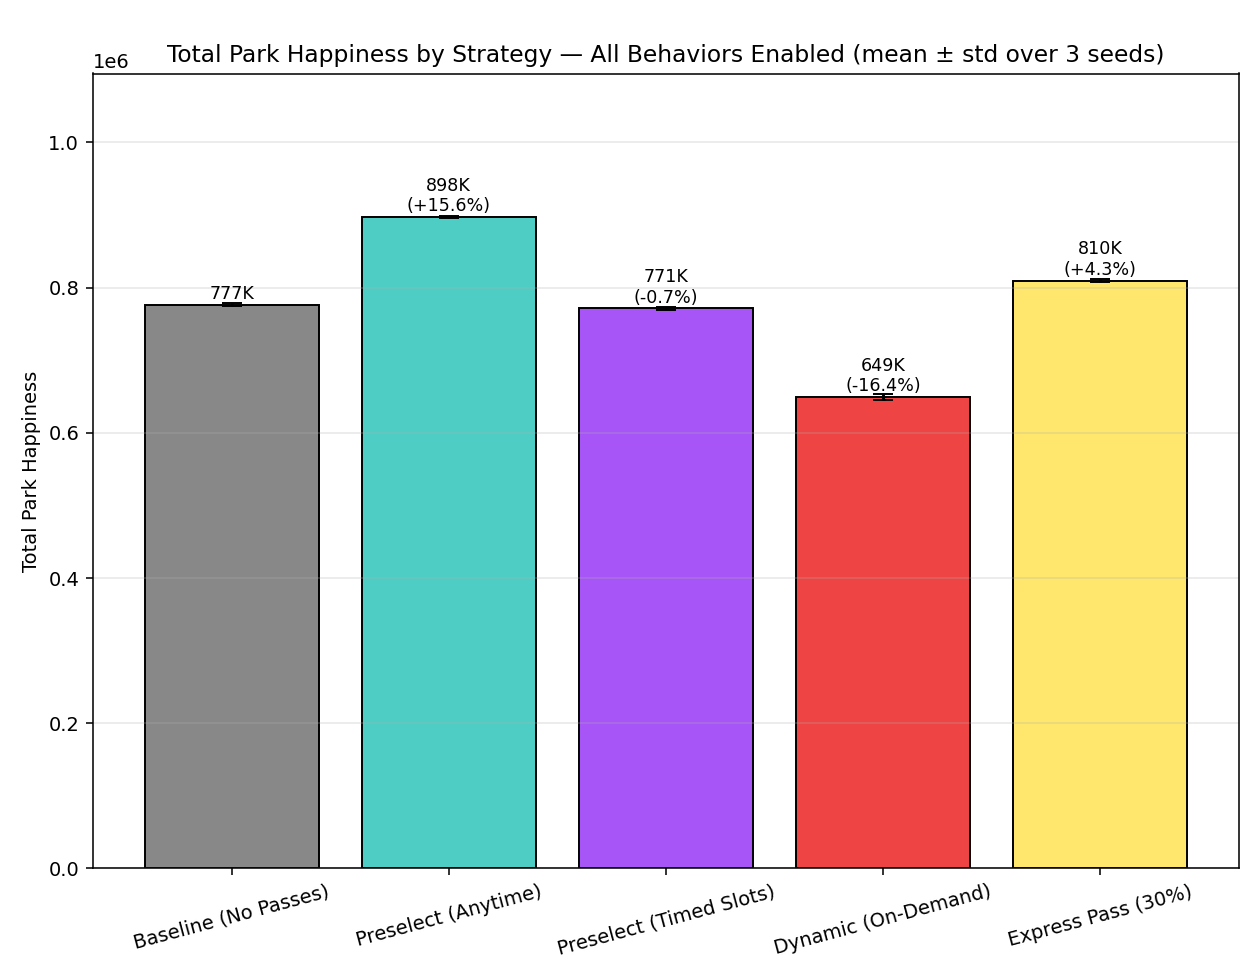
\includegraphics[width=0.9\linewidth]{behaviors_comparison_happiness.png}
\caption{Total park happiness by strategy under bounded rationality (all behaviors enabled, 3-seed mean $\pm$ std).}
\label{fig:behaviors-comparison}
\end{figure}

\subsection{Express Pass Participation Sweep}

We sweep Express Pass adoption $\beta \in \{0, 10, 20, \ldots, 100\}\%$ at seed 42 to characterize how participation rate affects system outcomes. Figure~\ref{fig:express-sweep} (rational) and Figure~\ref{fig:express-sweep-behaviors} (bounded-rational) show heatmaps of holder and non-holder utility distributions plus a line plot of summary statistics.

\begin{figure}[H]
\centering
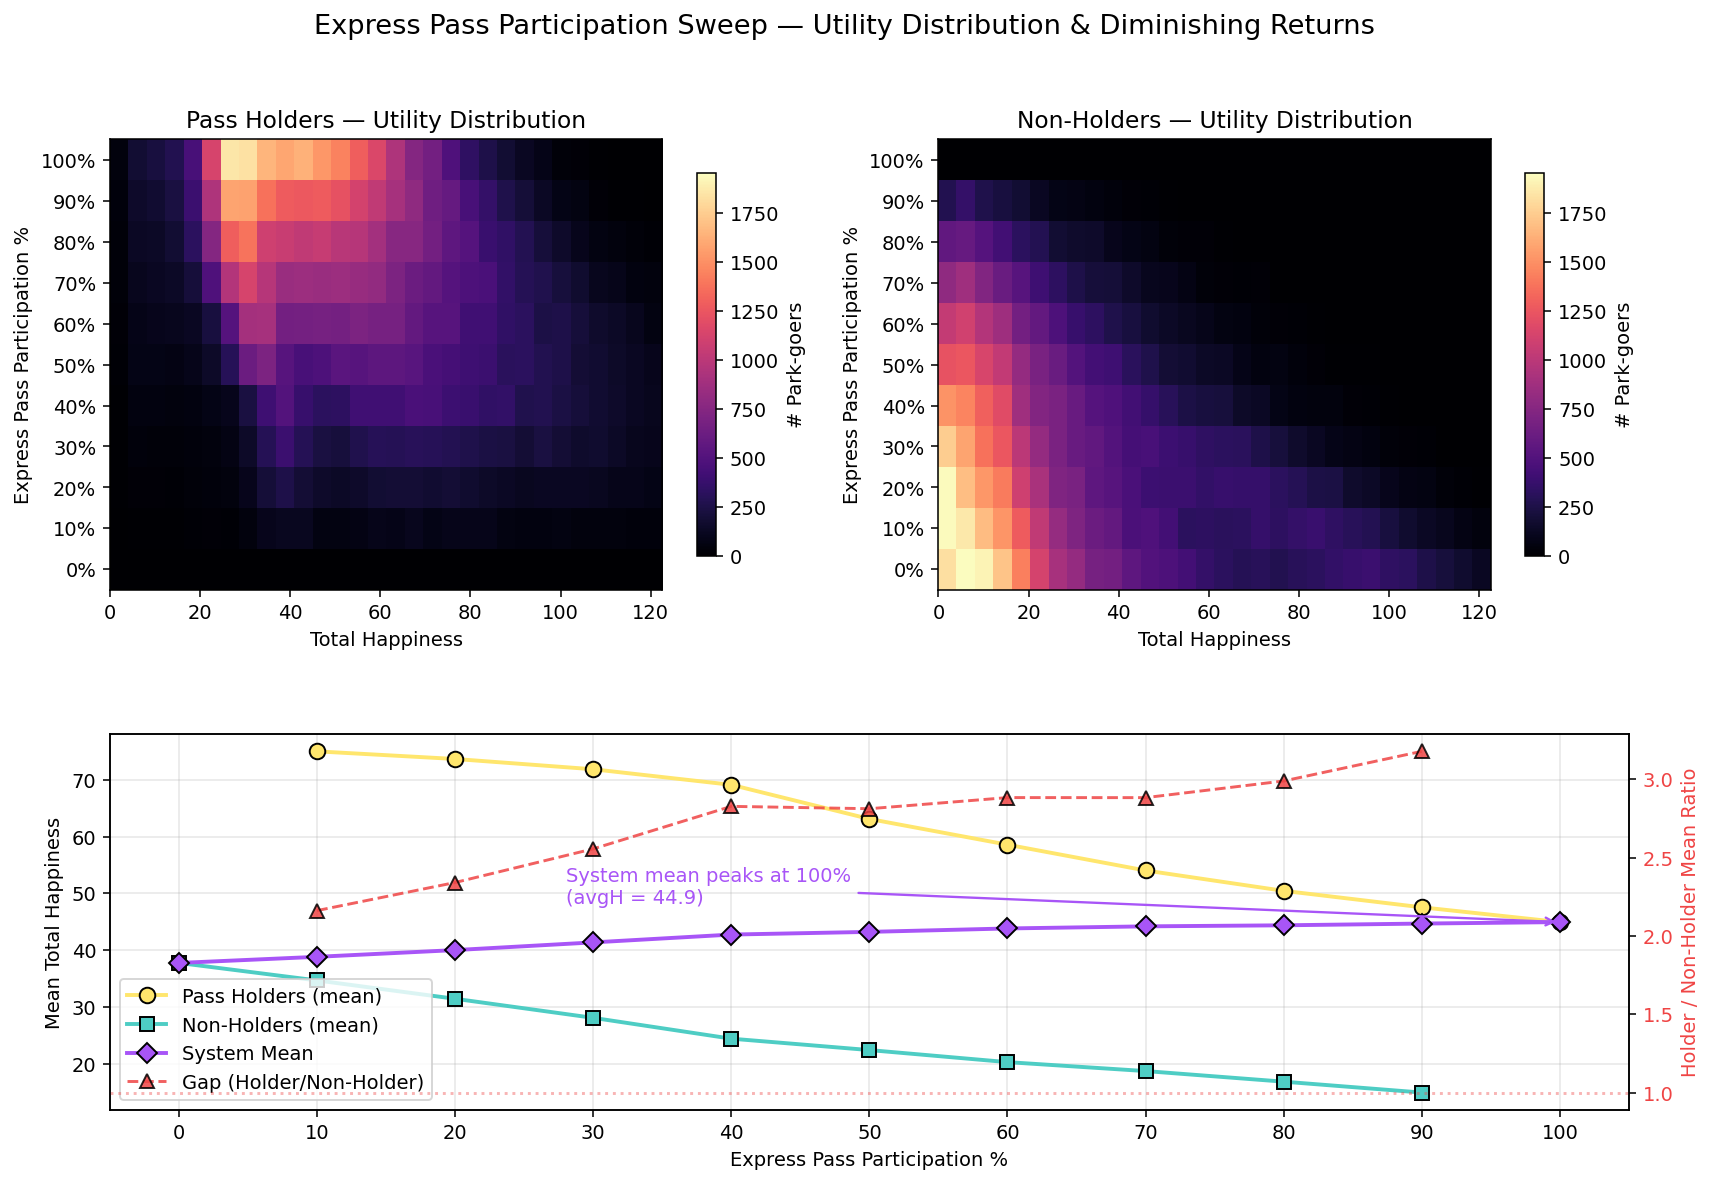
\includegraphics[width=0.95\linewidth]{express_sweep.png}
\caption{Express Pass participation sweep, perfectly-rational agents. System mean happiness rises monotonically with adoption; the holder/non-holder gap also rises monotonically.}
\label{fig:express-sweep}
\end{figure}

\begin{figure}[H]
\centering
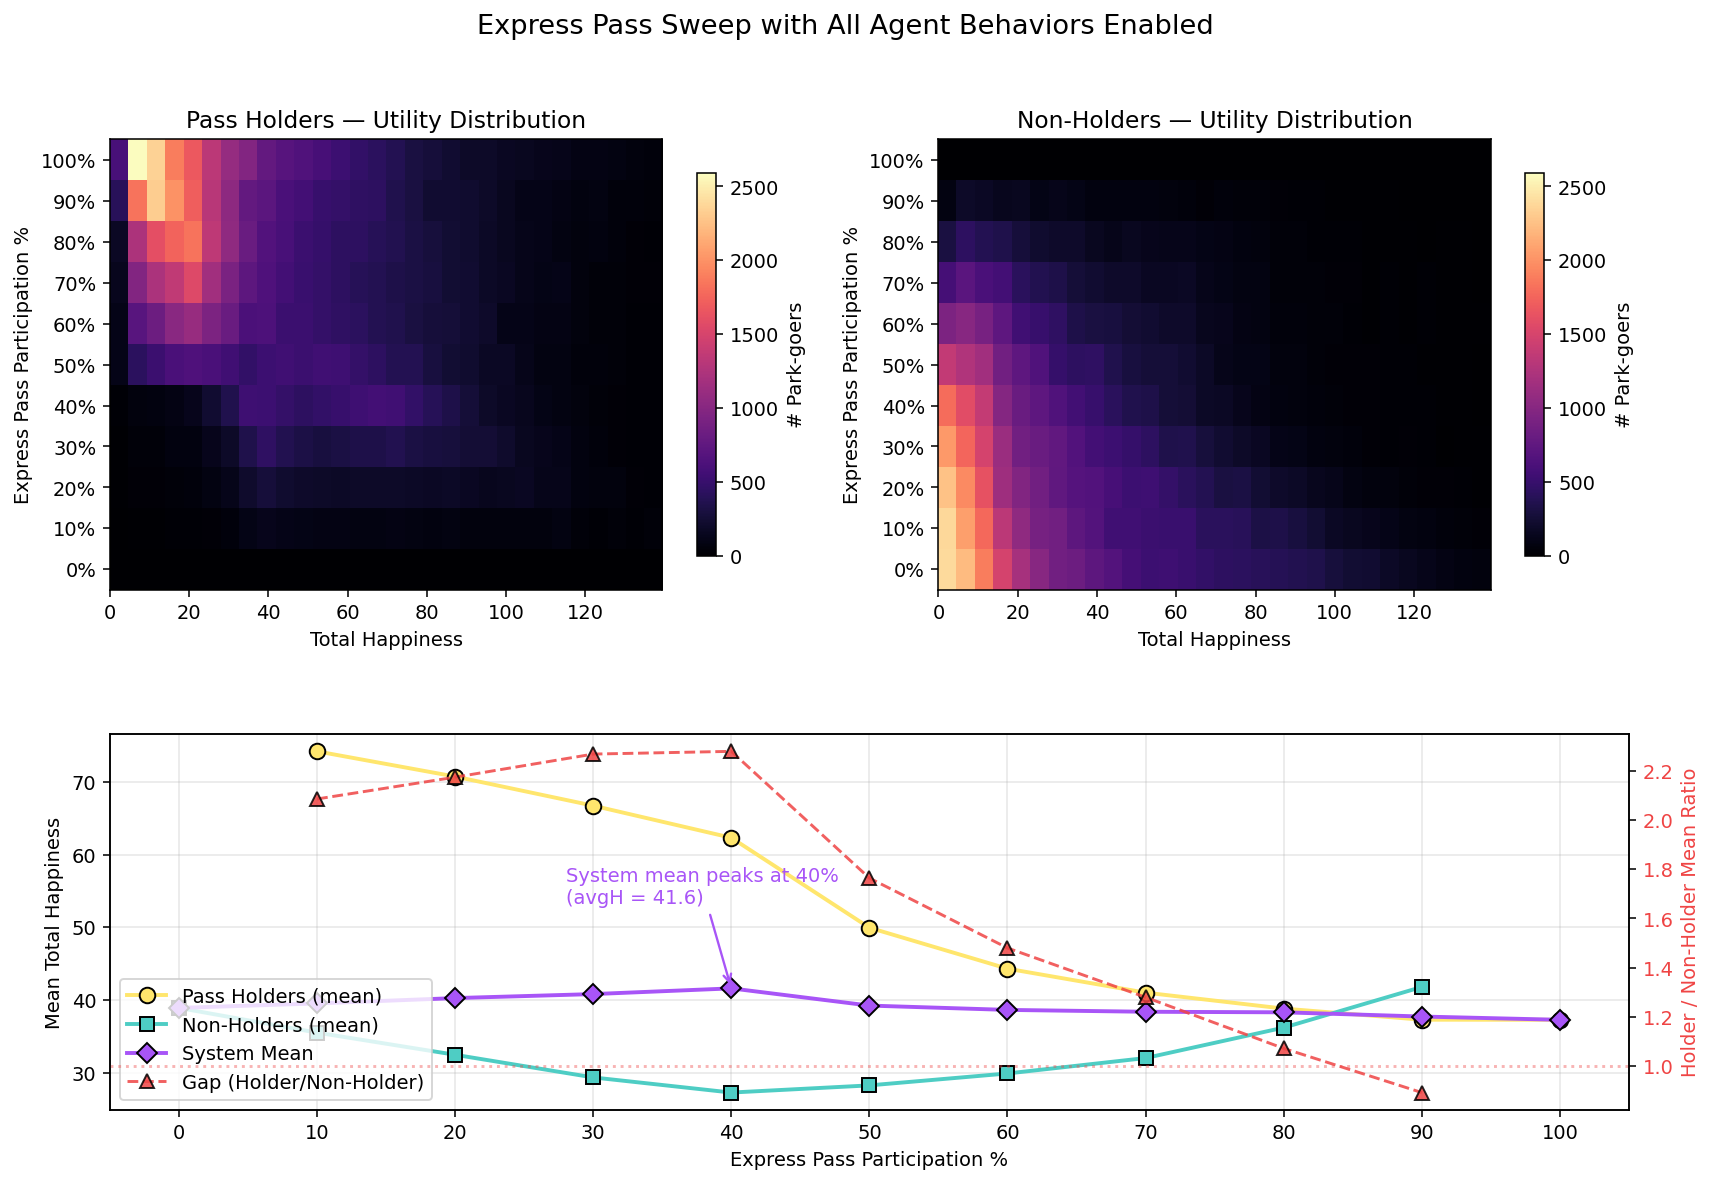
\includegraphics[width=0.95\linewidth]{behaviors_express_sweep.png}
\caption{Express Pass participation sweep, all behaviors enabled. Note the diminishing-returns inflection at $\beta = 40\%$; the strategy underperforms the no-passes baseline at $\beta = 100\%$.}
\label{fig:express-sweep-behaviors}
\end{figure}

The two regimes produce qualitatively different system-mean curves:
\begin{itemize}[nosep]
    \item \textbf{Perfect rationality:} Express system mean rises monotonically from 37.74 at $\beta = 0\%$ to 44.94 at $\beta = 100\%$.
    \item \textbf{Bounded rationality:} Express system mean peaks at $\beta = 40\%$ (avgH $= 41.60$) and \emph{declines} at higher adoption, ending at 37.36 at $\beta = 100\%$ --- below the no-passes baseline of 39.01.
\end{itemize}

The rationality assumption thus determines whether Express has diminishing returns at all. Under perfect rationality, more adoption is always better. Under realistic agent behavior, there is a clear optimal participation rate near 40\%.

\subsection{Paid Preselect Adoption Sweep}

We perform the same sweep for paid Preselect adoption $\alpha \in \{0, 10, 20, \ldots, 100\}\%$. Figures \ref{fig:preselect-sweep} and \ref{fig:preselect-sweep-behaviors} present the composite figures.

\begin{figure}[H]
\centering
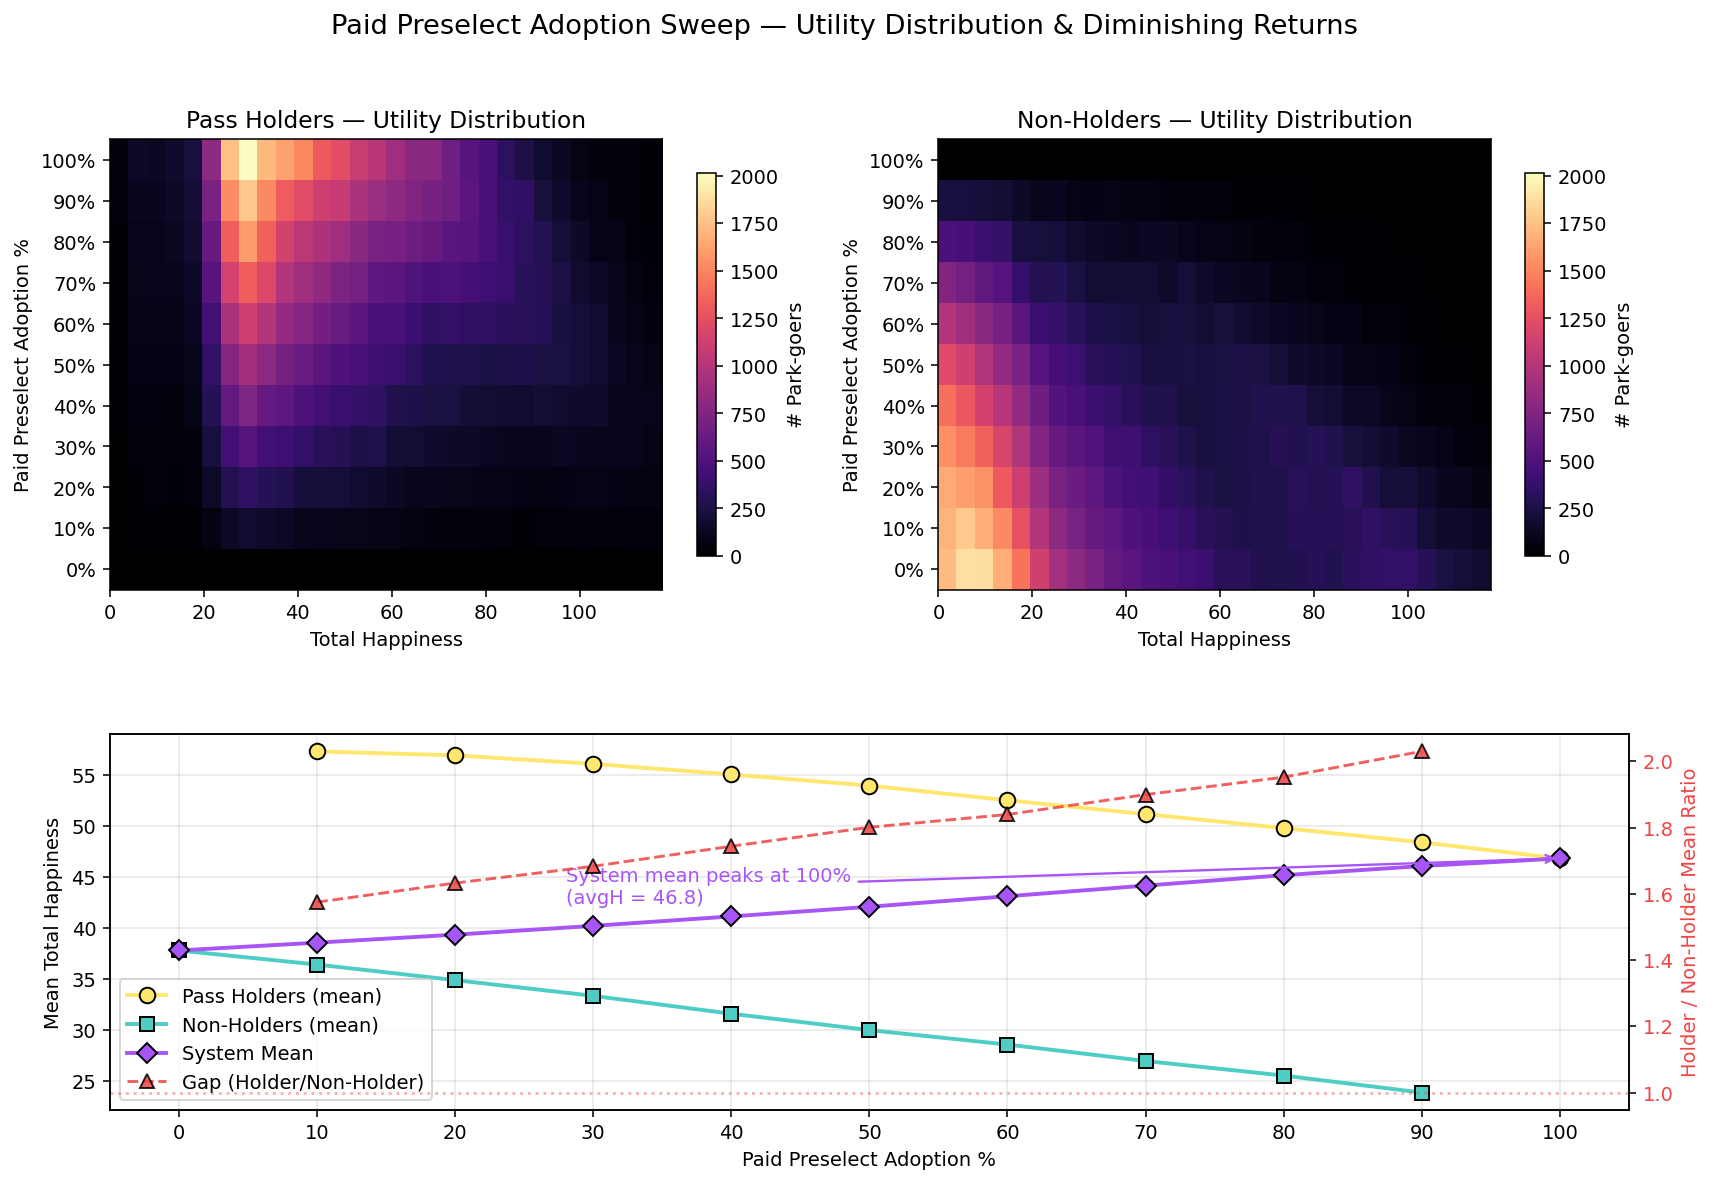
\includegraphics[width=0.95\linewidth]{preselect_paid_sweep.png}
\caption{Paid Preselect adoption sweep, perfectly-rational agents. System mean rises monotonically; gap ratio is uniformly smaller than Express at every adoption level.}
\label{fig:preselect-sweep}
\end{figure}

\begin{figure}[H]
\centering
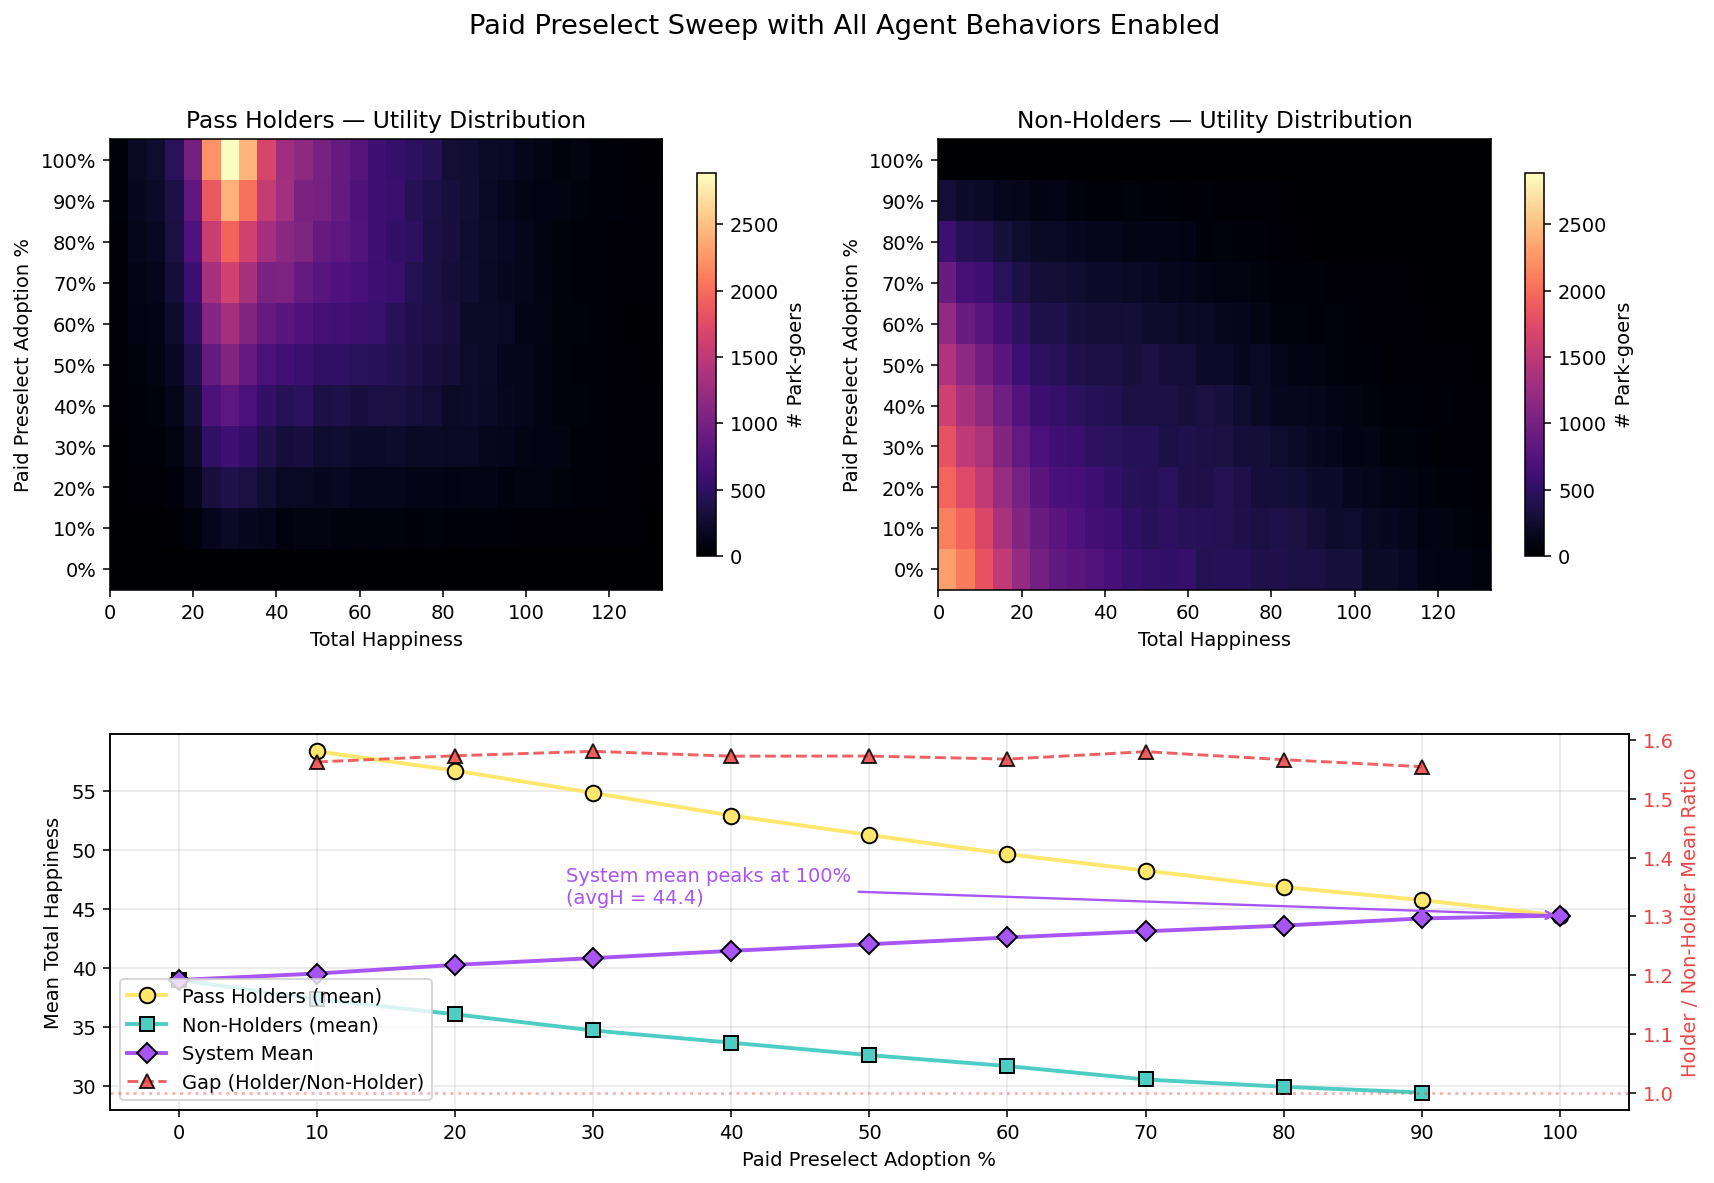
\includegraphics[width=0.95\linewidth]{behaviors_preselect_paid_sweep.png}
\caption{Paid Preselect adoption sweep, all behaviors enabled. Unlike Express, Preselect remains monotonically increasing under bounded rationality.}
\label{fig:preselect-sweep-behaviors}
\end{figure}

In contrast to Express, paid Preselect monotonically improves with adoption \emph{in both regimes}:
\begin{itemize}[nosep]
    \item \textbf{Perfect rationality:} system mean rises from 37.74 at $\alpha = 0\%$ to 46.78 at $\alpha = 100\%$.
    \item \textbf{Bounded rationality:} system mean rises from 38.93 at $\alpha = 0\%$ to 44.47 at $\alpha = 100\%$.
\end{itemize}

The targeted top-3 mechanic does not exhibit the saturation that Express does. Because each agent's three passes target different rides (heterogeneous personal preferences), the priority queue load is naturally distributed across attractions rather than concentrating at the most popular one.

\subsection{Fairness Analysis}

For Express and paid Preselect (the two strategies with non-uniform access), we measure the holder/non-holder gap ratio $G(\rho) = \bar{h}_{\text{holder}}(\rho) / \bar{h}_{\text{non-holder}}(\rho)$ at adoption rate $\rho$. A ratio of 1.0 means holders and non-holders achieve equal happiness on average; higher means holders benefit more.

\begin{table}[H]
\centering
\begin{tabular}{ccccc}
\toprule
\textbf{Adoption \%} & \textbf{Express} & \textbf{Preselect} & \textbf{Express} & \textbf{Preselect} \\
& \textbf{(Rational)} & \textbf{(Rational)} & \textbf{(Behaviors)} & \textbf{(Behaviors)} \\
\midrule
30\% & 2.56$\times$ & 1.68$\times$ & 2.27$\times$ & 1.58$\times$ \\
50\% & 2.81$\times$ & 1.80$\times$ & 1.77$\times$ & 1.57$\times$ \\
90\% & 3.17$\times$ & 2.03$\times$ & 0.90$\times$ & 1.54$\times$ \\
\bottomrule
\end{tabular}
\caption{Holder/non-holder happiness gap ratio at varying adoption rates. Lower ratios indicate more equitable outcomes.}
\label{tab:fairness}
\end{table}

\textbf{Two findings:}
\begin{itemize}[nosep]
    \item \textbf{Preselect is uniformly more equitable than Express} at every adoption level under both rationality regimes. The targeted top-3 mechanism distributes pass benefits more thinly per holder, while Express's blanket access concentrates benefits in a smaller holder population.
    \item \textbf{Express's gap inverts at 90\% under bounded rationality} (0.90$\times$): non-holders earn higher happiness than holders. The mechanism: at very high Express adoption, the priority queue at popular rides becomes saturated, and \texttt{info\_restricted} agents cannot accurately perceive this. Pass holders pile into already-overloaded priority queues, while the residual non-holders --- effectively forced to substitute toward less popular rides --- experience less congestion. This is a model artifact in the sense that we do not believe non-holders truly benefit from being "outside" Express in real parks; it reflects how compounded informational frictions degrade an over-saturated priority queue.
\end{itemize}

%----------------------------------------------------------------------
\section{Discussion}
%----------------------------------------------------------------------

The results support five interpretive claims that translate the experiments into operational and theoretical takeaways.

\textbf{1. Targeting beats blanket access.} Across every adoption level we tested, Preselect's targeted top-3 mechanism produces higher system happiness and a smaller fairness gap than Express's blanket access. The intuition is straightforward: a pass is most valuable when applied to a ride the agent has high personal preference for. Preselect concentrates pass usage exactly where this marginal benefit is largest. Express scatters pass usage across whatever ride the agent walks up to first, including rides with low personal preference where the marginal benefit of skipping is small. The same number of skips, applied in different patterns, produce materially different system outcomes.

\textbf{2. The rationality price varies dramatically across mechanisms.} An operations team choosing among virtual queue strategies must weight not only efficiency under perfect rationality but robustness to imperfect rationality. Express loses 0.41 happiness under bounded rationality; Dynamic loses 6.35. This is roughly a 15-fold difference in robustness. Mechanisms whose decision rule requires sophisticated wait-time judgment (Dynamic's 30-minute threshold; Timed's location-and-time matching) collapse when agents have stale or imperfect information. Mechanisms with simple decision rules (Express's "always skip"; Preselect's "use these three") retain their efficiency. The robustness profile thus deserves first-class consideration in deployment decisions, not merely as a footnote.

\textbf{3. Free FastPass+ was welfare-optimal but politically unsustainable.} The free Preselect (Anytime) configuration we modeled --- the closest analogue to Disney's pre-2021 FastPass+ system --- produces the highest system happiness in our experiments. Its real-world failure had little to do with welfare mathematics: the issue was booking-window arbitrage, where sophisticated planners booked the most desirable passes 60 days in advance, creating a perceived inequity between "savvy" and "casual" guests. Disney's replacement (Lightning Lane, paid and time-locked) traded efficiency for equity-of-access --- a value judgment, not a Pareto improvement. Our data is consistent with this read: the free version was efficient; the paid version is more "fair" in the sense that opt-out is voluntary rather than knowledge-gated.

\textbf{4. Universal Express's design is more robust than Disney Lightning Lane's.} Lightning Lane bundles Preselect (timed) with paid access. Our \texttt{preselect\_timed} strategy --- a clean implementation of timed-slot mechanics --- gains only +1.3\% over baseline under perfect rationality and \emph{drops below baseline} under bounded rationality (Table~\ref{tab:behaviors-strategies}). Universal Express's "always-on" rule, despite appearing less sophisticated, is robust to the same agent imperfections that destroy timed slots. This contradicts the casual intuition that Disney's "more sophisticated" pricing system is also "better designed."

\textbf{5. Universal's Express pricing approximately implements the welfare optimum.} Our bounded-rational Express sweep peaks at $\beta \approx 40\%$ adoption. Universal sells Express Pass at \$80--300 per day (variable by date and demand), and reported adoption rates fall in the 25--35\% range during normal-demand periods. The pricing pressure that limits adoption naturally lands the system near its welfare-maximizing operating point --- a Pigovian-style outcome achieved through revenue management rather than explicit Pigovian taxation. Without modeling pricing explicitly, we have inadvertently confirmed that real-world pricing is approximately doing the right thing.

%----------------------------------------------------------------------
\section{Limitations}
%----------------------------------------------------------------------

We document the modeling choices that constrain the interpretation of these findings:

\begin{itemize}[nosep]
    \item \textbf{Theoretical-capacity assumption.} All rides are modeled as running at full theoretical hourly capacity throughout the day. Real parks experience downtime and reduced throughput; effects on relative strategy ranking should be small but absolute happiness numbers are upper bounds.
    \item \textbf{No multi-day visitors.} Agents have a single arrival/departure within one operating day. Real parks have multi-day pass holders whose strategy may differ on day 2.
    \item \textbf{No group dynamics.} Each agent makes independent decisions. Real visitors travel in family or friend groups whose collective decisions are slower and less individually-optimal.
    \item \textbf{No weather, ride breakdowns, or seasonal effects.}
    \item \textbf{Single-source data} for waits and capacity (thrill-data.com). Capacity is the published theoretical maximum; observed throughput is typically lower.
    \item \textbf{Eating threshold $\mathcal{N}(225, 15)$ minutes is an estimate}, not calibrated to data on real meal-time behavior.
    \item \textbf{Pricing is implicit.} We use participation rate $\alpha$ or $\beta$ as a proxy for willingness-to-pay; we do not compute or sweep an explicit Pigovian toll.
    \item \textbf{Pass-holder priority-queue wait under \texttt{info\_restricted}} is approximated as zero (the stale wait-time board does not expose priority queue length to bounded-rational agents). This is a small lag we accept; live-information agents see the priority queue length correctly.
    \item \textbf{The \texttt{pending\_arrivals} counter tracks only non-pass commitments}, introducing a small lag in pass-holder traffic visibility within a single timestep.
    \item \textbf{No demand-side learning.} Agents do not adjust expectations based on prior visits; in real life, repeat visitors learn which rides are typically crowded.
\end{itemize}

%----------------------------------------------------------------------
\section{Conclusions and Recommendations}
%----------------------------------------------------------------------

We close with three operational recommendations and a statement of contribution.

\textbf{Recommendation 1: For maximum aggregate visitor utility under realistic rationality, deploy a paid Preselect system.} Paid Preselect at 100\% adoption produces +18\% system happiness above baseline under bounded-rational agents, vs +9\% for Express @ 30\% and +1\% for timed slots. Targeted top-3 selection scales gracefully across adoption levels and is robust to imperfect agent decisions.

\textbf{Recommendation 2: If a Preselect-like system is politically infeasible, Express @ 30\% is the second-best deployable choice.} Universal-style Express produces meaningful efficiency gains, is robust to imperfect agents, and the pricing mechanism naturally targets the welfare-maximizing adoption rate. The fairness gap is larger than under Preselect, but the mechanism is operationally simpler and politically more stable than universal-access alternatives.

\textbf{Recommendation 3: Avoid threshold-based dynamic systems at any scale that includes substantial information friction.} Dynamic's efficiency under perfect rationality (+22\%) collapses to baseline-equivalent under realistic rationality (+1\%), because the 30-minute wait threshold is sensitive to perception accuracy that bounded-rational agents do not have. The same applies to timed-slot systems, which fall below baseline once agents have imperfect information.

\textbf{Statement of contribution.} This work demonstrates that the \emph{robustness profile} of a virtual queue strategy under bounded rationality is as important to its real-world performance as its efficiency under perfect rationality. The strategy ranking changes when agents become imperfect, with Express climbing and Dynamic collapsing; this re-ordering is large enough to invert deployment decisions. Targeted-allocation mechanisms (Preselect-style) outperform blanket-allocation mechanisms (Express-style) on both efficiency and equity dimensions across all adoption levels and all rationality regimes we tested. Universal Orlando's empirical Express pricing approximately implements the welfare-maximizing adoption level for its mechanism, suggesting that revenue-driven adoption controls can mimic Pigovian externality pricing in this domain without explicit calculation.

%----------------------------------------------------------------------
\section{Appendix: Code, Figure, and Data Index}
%----------------------------------------------------------------------

\textbf{Source code repository.} The full source code, simulation engine, sweep scripts, figures, and data files for this project are available at:
\begin{center}
\url{https://github.com/Belugaluga2/Networks-Project-ORF387}
\end{center}

\noindent The simulation engine lives in \texttt{simulation.py}, the network model in \texttt{park\_model.py}, and the on-demand backend server in \texttt{server.py}.

\subsection*{Reproducibility Index}

Each results section in this report is generated by a dedicated script that consumes the simulation engine and emits both a CSV of summary statistics and PNG figures into the \texttt{figures/} directory.

\begin{itemize}[leftmargin=*, itemsep=4pt]
    \item \textbf{Strategy comparison (rational).}
        Script: \texttt{generate\_report\_data.py}.
        Data: \texttt{results.csv}.
    \item \textbf{Strategy comparison (all behaviors).}
        Script: \texttt{generate\_report\_data\_behaviors.py}.
        Data: \texttt{behaviors\_results.csv}.
    \item \textbf{Express adoption sweep (rational).}
        Script: \texttt{express\_sweep.py}.
        Data: \texttt{express\_sweep\_results.csv}.
    \item \textbf{Express adoption sweep (all behaviors).}
        Script: \texttt{behaviors\_express\_sweep.py}.
        Data: \texttt{behaviors\_express\_sweep\_results.csv}.
    \item \textbf{Paid Preselect adoption sweep (rational).}
        Script: \texttt{preselect\_paid\_sweep.py}.
        Data: \texttt{preselect\_paid\_sweep\_results.csv}.
    \item \textbf{Paid Preselect adoption sweep (all behaviors).}
        Script: \texttt{behaviors\_preselect\_paid\_sweep.py}.
        Data: \texttt{behaviors\_preselect\_paid\_sweep\_results.csv}.
\end{itemize}

\subsection*{Figure Naming Convention}

All figures referenced in this report are stored in the \texttt{figures/} directory of the project repository. The naming convention is:

\begin{itemize}[leftmargin=*, itemsep=4pt]
    \item \textbf{Per-strategy figures} (rational): \texttt{\{strategy\}\_histogram.png}, \texttt{\{strategy\}\_queues.png}, \texttt{\{strategy\}\_population.png}.
    \item \textbf{Per-strategy figures} (with all behaviors): same names prefixed with \texttt{behaviors\_}.
    \item \textbf{Cross-strategy comparison charts}: \texttt{comparison\_happiness.png}, \texttt{comparison\_avg\_metrics.png}, \texttt{comparison\_distributions.png}, and the same prefixed with \texttt{behaviors\_} for the bounded-rational variants.
    \item \textbf{Composite sweep figures}: \texttt{express\_sweep.png}, \texttt{behaviors\_express\_sweep.png}, \texttt{preselect\_paid\_sweep.png}, \texttt{behaviors\_preselect\_paid\_sweep.png}.
\end{itemize}

\end{document}
